\section{Travaux Pratiques --- Supervision et Gestion de
Réseaux}\label{travaux-pratiques-supervision-et-gestion-de-ruxe9seaux}

\subsection{Mise en œuvre d'une architecture complète de supervision et
de
sécurité}\label{mise-en-ux153uvre-dune-architecture-compluxe8te-de-supervision-et-de-suxe9curituxe9}

\textbf{Auteur :} Razafindrabetany Roger Marius\\
\textbf{Enseignant :} Tommy Montégu\\
\textbf{Formation :} ESIROI --- 4A Informatique\\
\textbf{Date :} Février 2026

\subsection{Table des matières}\label{table-des-matiuxe8res}

\hyperref[1-infrastructure-du-ruxe9seau]{Infrastructure du réseau}
\hyperref[2-configuration-snmp-sur-les-serveurs-cibles]{Configuration
SNMP sur les serveurs cibles}
\hyperref[3-installation-et-configuration-du-serveur-de-supervision]{Installation
et configuration du serveur de supervision (srv-monitoring)}
\hyperref[4-installation-et-configuration-du-serveur-linux]{Installation
et configuration du serveur Linux (srv-linux)}
\hyperref[5-configuration-du-pare-feu-pfsense]{Configuration du pare-feu
pfSense} \hyperref[6-configuration-du-serveur-windows]{Configuration du
serveur Windows (AK-DC)}
\hyperref[7-supervision-avec-zabbix]{Supervision avec Zabbix}
\hyperref[8-supervision-avancuxe9e--sondes-et-alertes]{Supervision
avancée --- Sondes et alertes}
\hyperref[9-siem-wazuh--centralisation-des-logs]{SIEM Wazuh ---
Centralisation des logs}
\hyperref[10-simulation-dune-attaque-par-force-brute-ssh]{Simulation
d'une attaque par force brute SSH} \hyperref[11-conclusion]{Conclusion}

\subsection{Infrastructure du réseau}\label{infrastructure-du-ruxe9seau}

\subsubsection{Schéma réseau}\label{schuxe9ma-ruxe9seau}

L'infrastructure déployée dans ce TP repose sur quatre machines
virtuelles hébergées sous VirtualBox, interconnectées via un réseau
interne en mode Bridge sur le sous-réseau \texttt{192.168.1.0/24}. Le
serveur de supervision centralise toutes les données collectées sur les
autres machines.

\pandocbounded{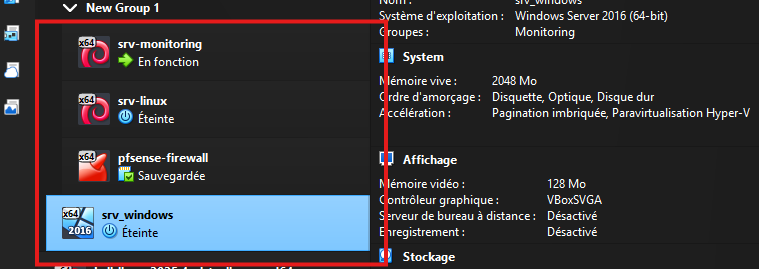
\includegraphics[keepaspectratio,alt={Liste des machines virtuelles déployées dans VirtualBox}]{images/vms_list.png}}
\emph{Figure 1 --- Liste des machines virtuelles déployées dans
VirtualBox}

\subsubsection{Plan d'adressage IP}\label{plan-dadressage-ip}

{\def\LTcaptype{none} % do not increment counter
\begin{longtable}[]{@{}
  >{\raggedright\arraybackslash}p{(\linewidth - 8\tabcolsep) * \real{0.2000}}
  >{\raggedright\arraybackslash}p{(\linewidth - 8\tabcolsep) * \real{0.2000}}
  >{\raggedright\arraybackslash}p{(\linewidth - 8\tabcolsep) * \real{0.2000}}
  >{\raggedright\arraybackslash}p{(\linewidth - 8\tabcolsep) * \real{0.2000}}
  >{\raggedright\arraybackslash}p{(\linewidth - 8\tabcolsep) * \real{0.2000}}@{}}
\toprule\noalign{}
\begin{minipage}[b]{\linewidth}\raggedright
Nom d'hôte
\end{minipage} & \begin{minipage}[b]{\linewidth}\raggedright
Rôle
\end{minipage} & \begin{minipage}[b]{\linewidth}\raggedright
Système d'exploitation
\end{minipage} & \begin{minipage}[b]{\linewidth}\raggedright
Adresse IP
\end{minipage} & \begin{minipage}[b]{\linewidth}\raggedright
Services
\end{minipage} \\
\midrule\noalign{}
\endhead
\bottomrule\noalign{}
\endlastfoot
srv-monitoring & Supervision centrale + SIEM & Debian 12 (GNOME) &
192.168.1.100 & Zabbix Server, Wazuh All-in-One, Apache, MariaDB \\
srv-linux & Serveur applicatif & Debian 12 & 192.168.1.10 & Nginx (port
80), Agent Zabbix, Agent Wazuh, SNMP \\
AK-DC & Contrôleur de domaine & Windows Server 2019 & 192.168.1.11 &
Active Directory, Agent Zabbix, Agent Wazuh \\
firewall & Pare-feu / Routeur & pfSense 2.7.0 & 192.168.1.1 & SNMP,
Syslog vers Wazuh \\
\end{longtable}
}

\subsubsection{Caractéristiques du
réseau}\label{caractuxe9ristiques-du-ruxe9seau}

\begin{itemize}
\tightlist
\item
  \textbf{Réseau :} 192.168.1.0/24
\item
  \textbf{Masque :} 255.255.255.0
\item
  \textbf{Plage IP :} 192.168.1.1 -- 192.168.1.254
\item
  \textbf{Type de réseau VirtualBox :} Bridge Adapter (accès au réseau
  physique)
\item
  \textbf{Accès Internet :} via une deuxième interface en mode NAT (pour
  les téléchargements)
\end{itemize}

\subsubsection{Architecture de
supervision}\label{architecture-de-supervision}

\begin{verbatim}
srv-monitoring (192.168.1.100)
  ├── Supervision via Agent Zabbix ──► srv-linux (192.168.1.10)
  ├── Supervision via Agent Zabbix ──► AK-DC (192.168.1.11)
  ├── Supervision via SNMP v2c     ──► firewall (192.168.1.1)
  ├── Collecte logs Wazuh          ──► srv-linux (agent Wazuh)
  ├── Collecte logs Wazuh          ──► AK-DC (agent Wazuh)
  └── Collecte syslog              ──► firewall (syslog UDP 514)
\end{verbatim}

\subsection{Configuration SNMP sur les serveurs
cibles}\label{configuration-snmp-sur-les-serveurs-cibles}

\subsubsection{Choix de l'outil de supervision :
Zabbix}\label{choix-de-loutil-de-supervision-zabbix}

\textbf{Justification du choix :} Zabbix a été retenu pour ce TP pour
les raisons suivantes : - \textbf{Open source} et sans licence
commerciale, adapté à un environnement académique. - \textbf{Support
natif de SNMP} (v1, v2c, v3) sans plugin supplémentaire. -
\textbf{Templates prêts à l'emploi} pour Linux, Windows, pfSense et
équipements réseau. - \textbf{Agent natif} léger disponible pour Linux
et Windows. - \textbf{Interface web} complète pour la configuration et
la visualisation. - \textbf{Base de données} MariaDB/MySQL nativement
supportée.

Centreon aurait été une alternative viable mais requiert plus de
ressources et une courbe d'apprentissage plus importante.

\subsubsection{SNMP sur srv-linux
(192.168.1.10)}\label{snmp-sur-srv-linux-192.168.1.10}

\paragraph{Installation}\label{installation}

\begin{Shaded}
\begin{Highlighting}[]
\FunctionTok{sudo}\NormalTok{ apt update}
\FunctionTok{sudo}\NormalTok{ apt install snmpd snmp }\AttributeTok{{-}y}
\end{Highlighting}
\end{Shaded}

\paragraph{\texorpdfstring{Configuration de
\texttt{/etc/snmp/snmpd.conf}}{Configuration de /etc/snmp/snmpd.conf}}\label{configuration-de-etcsnmpsnmpd.conf}

\begin{Shaded}
\begin{Highlighting}[]
\CommentTok{\# Écouter sur toutes les interfaces}
\DataTypeTok{agentAddress udp:161,udp6:}\KeywordTok{[::1]}\DataTypeTok{:161}

\CommentTok{\# Communauté en lecture seule accessible depuis le réseau de supervision}
\DataTypeTok{rocommunity public 192.168.1.0/24}

\CommentTok{\# Informations système}
\DataTypeTok{sysLocation "Sitting on the Dock of the Bay"}
\DataTypeTok{sysContact "Me \textless{}admin@esiroi.local\textgreater{}"}
\end{Highlighting}
\end{Shaded}

\paragraph{Démarrage et
vérification}\label{duxe9marrage-et-vuxe9rification}

\begin{Shaded}
\begin{Highlighting}[]
\FunctionTok{sudo}\NormalTok{ systemctl restart snmpd}
\FunctionTok{sudo}\NormalTok{ systemctl enable snmpd}
\FunctionTok{sudo}\NormalTok{ netstat }\AttributeTok{{-}tuln} \KeywordTok{|} \FunctionTok{grep}\NormalTok{ 161}
\end{Highlighting}
\end{Shaded}

\paragraph{Test de connectivité et
SNMP}\label{test-de-connectivituxe9-et-snmp}

\pandocbounded{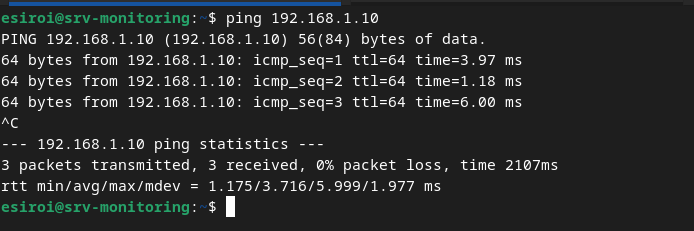
\includegraphics[keepaspectratio,alt={Test de connectivité entre srv-monitoring et srv-linux}]{images/ping_from_srv_monitoring_to_srv_linux.png}}
\emph{Figure 2 --- Test de connectivité (ping) entre srv-monitoring et
srv-linux}

\paragraph{Test snmpwalk depuis
srv-monitoring}\label{test-snmpwalk-depuis-srv-monitoring}

\begin{Shaded}
\begin{Highlighting}[]
\ExtensionTok{snmpwalk} \AttributeTok{{-}v}\NormalTok{ 2c }\AttributeTok{{-}c}\NormalTok{ public 192.168.1.10}
\end{Highlighting}
\end{Shaded}

\textbf{Résultat obtenu :}

\begin{verbatim}
iso.3.6.1.2.1.1.1.0 = STRING: "Linux srv-linux 6.1.0-43-amd64 #1 SMP PREEMPT_DYNAMIC Debian 6.1.162-1 (2026-02-08) x86_64"
iso.3.6.1.2.1.1.5.0 = STRING: "srv-linux"
...
\end{verbatim}

\pandocbounded{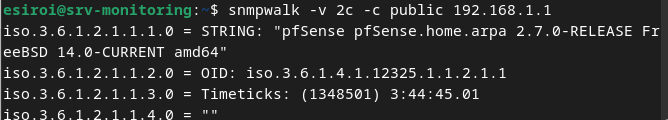
\includegraphics[keepaspectratio,alt={Résultat du snmpwalk sur le firewall pfSense}]{images/snmp_walk_on_pfsense_result.png}}
\emph{Figure 3 --- Résultat du snmpwalk sur le firewall pfSense}

\subsubsection{SNMP sur pfSense
(192.168.1.1)}\label{snmp-sur-pfsense-192.168.1.1}

La configuration SNMP sur pfSense s'effectue via l'interface web :

\begin{enumerate}
\def\labelenumi{\arabic{enumi}.}
\tightlist
\item
  Naviguer vers \textbf{Services → SNMP}
\item
  Cocher \textbf{Enable the SNMP Daemon}
\item
  Configurer :

  \begin{itemize}
  \tightlist
  \item
    \textbf{Polling Port :} 161
  \item
    \textbf{System Location :} ESIROI
  \item
    \textbf{System Contact :} admin@esiroi.local
  \item
    \textbf{Community String :} \texttt{public}
  \item
    \textbf{Bind Interfaces :} LAN
  \end{itemize}
\end{enumerate}

\pandocbounded{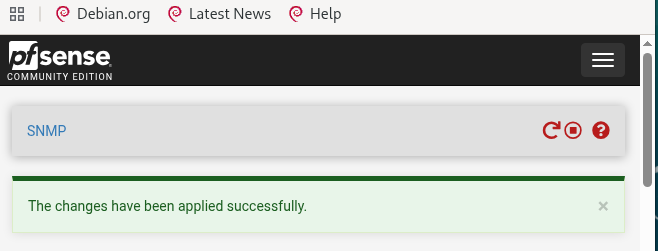
\includegraphics[keepaspectratio,alt={Interface SNMP activée sur pfSense}]{images/snmp_enabled_on_pfsense.png}}
\emph{Figure 4 --- Interface SNMP activée sur pfSense}

\textbf{Test de validation :}

\begin{Shaded}
\begin{Highlighting}[]
\ExtensionTok{snmpwalk} \AttributeTok{{-}v}\NormalTok{ 2c }\AttributeTok{{-}c}\NormalTok{ public 192.168.1.1}
\CommentTok{\# iso.3.6.1.2.1.1.1.0 = STRING: "pfSense pfSense.home.arpa 2.7.0{-}RELEASE FreeBSD 14.0{-}CURRENT amd64"}
\end{Highlighting}
\end{Shaded}

\subsection{Installation et configuration du serveur de
supervision}\label{installation-et-configuration-du-serveur-de-supervision}

\subsubsection{Prérequis --- Système
d'exploitation}\label{pruxe9requis-systuxe8me-dexploitation}

{\def\LTcaptype{none} % do not increment counter
\begin{longtable}[]{@{}ll@{}}
\toprule\noalign{}
Paramètre & Valeur \\
\midrule\noalign{}
\endhead
\bottomrule\noalign{}
\endlastfoot
OS & Debian GNU/Linux 12 (Bookworm) \\
Interface graphique & GNOME (task-gnome-desktop) \\
RAM & 4 Go \\
Stockage & 50 Go \\
Réseau & Bridge Adapter (192.168.1.100) + NAT (Internet) \\
\end{longtable}
}

\textbf{Note importante :} Après l'installation de GNOME, NetworkManager
a été désactivé pour éviter tout conflit avec systemd-networkd déjà en
place :

\begin{Shaded}
\begin{Highlighting}[]
\FunctionTok{sudo}\NormalTok{ systemctl stop NetworkManager}
\FunctionTok{sudo}\NormalTok{ systemctl disable NetworkManager}
\FunctionTok{sudo}\NormalTok{ systemctl restart systemd{-}networkd}
\end{Highlighting}
\end{Shaded}

\subsubsection{Installation de MariaDB}\label{installation-de-mariadb}

\begin{Shaded}
\begin{Highlighting}[]
\FunctionTok{sudo}\NormalTok{ apt install }\AttributeTok{{-}y}\NormalTok{ mariadb{-}server}
\FunctionTok{sudo}\NormalTok{ systemctl start mariadb}
\FunctionTok{sudo}\NormalTok{ systemctl enable mariadb}
\FunctionTok{sudo}\NormalTok{ mysql\_secure\_installation}
\end{Highlighting}
\end{Shaded}

\paragraph{Création de la base de données
Zabbix}\label{cruxe9ation-de-la-base-de-donnuxe9es-zabbix}

\begin{Shaded}
\begin{Highlighting}[]
\KeywordTok{CREATE} \KeywordTok{DATABASE}\NormalTok{ zabbix }\DataTypeTok{CHARACTER} \KeywordTok{SET}\NormalTok{ utf8mb4 COLLATE utf8mb4\_bin;}
\KeywordTok{CREATE} \FunctionTok{USER} \StringTok{\textquotesingle{}zabbix\textquotesingle{}}\NormalTok{@}\StringTok{\textquotesingle{}localhost\textquotesingle{}} \KeywordTok{IDENTIFIED} \KeywordTok{BY} \StringTok{\textquotesingle{}MotDePasseFort123!\textquotesingle{}}\NormalTok{;}
\KeywordTok{GRANT} \KeywordTok{ALL} \KeywordTok{PRIVILEGES} \KeywordTok{ON}\NormalTok{ zabbix.}\OperatorTok{*} \KeywordTok{TO} \StringTok{\textquotesingle{}zabbix\textquotesingle{}}\NormalTok{@}\StringTok{\textquotesingle{}localhost\textquotesingle{}}\NormalTok{;}
\KeywordTok{SET} \KeywordTok{GLOBAL}\NormalTok{ log\_bin\_trust\_function\_creators }\OperatorTok{=} \DecValTok{1}\NormalTok{;}
\NormalTok{QUIT;}
\end{Highlighting}
\end{Shaded}

\pandocbounded{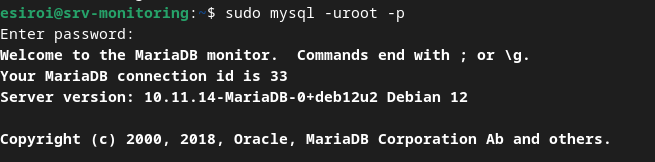
\includegraphics[keepaspectratio,alt={MariaDB installé et opérationnel}]{images/mariadb_installed_success.png}}
\emph{Figure 5 --- MariaDB installé et opérationnel}

\pandocbounded{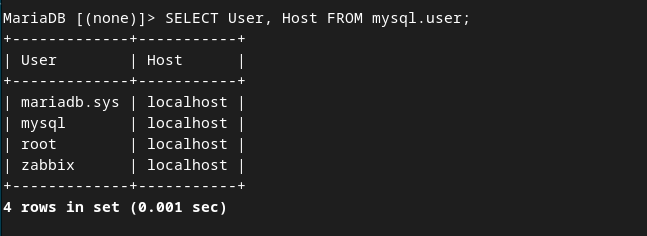
\includegraphics[keepaspectratio,alt={Schéma de la base de données Zabbix importé}]{images/database_schema.png}}
\emph{Figure 6 --- Schéma de la base de données Zabbix importé}

\pandocbounded{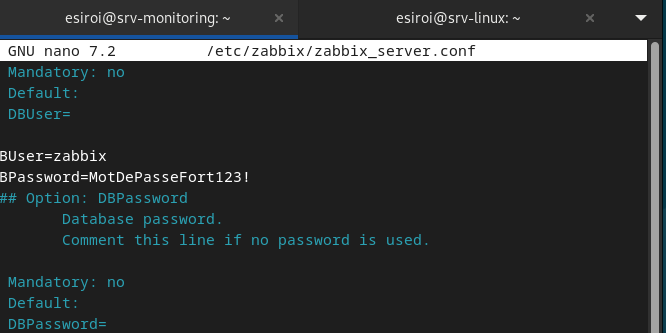
\includegraphics[keepaspectratio,alt={Mot de passe de la base de données configuré}]{images/db_password_added.png}}
\emph{Figure 7 --- Mot de passe de la base de données configuré dans
zabbix\_server.conf}

\subsubsection{Installation de Zabbix
Server}\label{installation-de-zabbix-server}

\paragraph{Ajout du dépôt Zabbix
6.4}\label{ajout-du-duxe9puxf4t-zabbix-6.4}

\begin{Shaded}
\begin{Highlighting}[]
\FunctionTok{wget}\NormalTok{ https://repo.zabbix.com/zabbix/6.4/debian/pool/main/z/zabbix{-}release/zabbix{-}release\_6.4{-}1+debian12\_all.deb}
\FunctionTok{sudo}\NormalTok{ dpkg }\AttributeTok{{-}i}\NormalTok{ zabbix{-}release\_6.4{-}1+debian12\_all.deb}
\FunctionTok{sudo}\NormalTok{ apt update}
\end{Highlighting}
\end{Shaded}

\paragraph{Installation des
composants}\label{installation-des-composants}

\begin{Shaded}
\begin{Highlighting}[]
\FunctionTok{sudo}\NormalTok{ apt install }\AttributeTok{{-}y}\NormalTok{ zabbix{-}server{-}mysql zabbix{-}frontend{-}php zabbix{-}apache{-}conf zabbix{-}sql{-}scripts zabbix{-}agent}
\end{Highlighting}
\end{Shaded}

\paragraph{Import du schéma initial}\label{import-du-schuxe9ma-initial}

\begin{Shaded}
\begin{Highlighting}[]
\FunctionTok{sudo}\NormalTok{ zcat /usr/share/zabbix{-}sql{-}scripts/mysql/server.sql.gz }\KeywordTok{|} \ExtensionTok{mysql} \AttributeTok{{-}uzabbix} \AttributeTok{{-}p}\NormalTok{ zabbix}
\FunctionTok{sudo}\NormalTok{ mysql }\AttributeTok{{-}uroot} \AttributeTok{{-}p} \AttributeTok{{-}e} \StringTok{"SET GLOBAL log\_bin\_trust\_function\_creators = 0;"}
\end{Highlighting}
\end{Shaded}

\paragraph{\texorpdfstring{Configuration de
\texttt{/etc/zabbix/zabbix\_server.conf}}{Configuration de /etc/zabbix/zabbix\_server.conf}}\label{configuration-de-etczabbixzabbix_server.conf}

\begin{Shaded}
\begin{Highlighting}[]
\DataTypeTok{DBPassword}\OtherTok{=}\StringTok{MotDePasseFort123!}
\end{Highlighting}
\end{Shaded}

\paragraph{Démarrage des services}\label{duxe9marrage-des-services}

\begin{Shaded}
\begin{Highlighting}[]
\FunctionTok{sudo}\NormalTok{ systemctl restart zabbix{-}server zabbix{-}agent apache2}
\FunctionTok{sudo}\NormalTok{ systemctl enable zabbix{-}server zabbix{-}agent apache2}
\end{Highlighting}
\end{Shaded}

\pandocbounded{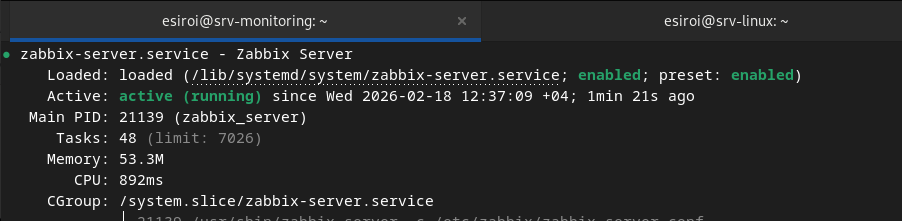
\includegraphics[keepaspectratio,alt={Service Zabbix Server actif et démarré}]{images/zabbix_server_enable_activated.png}}
\emph{Figure 8 --- Service Zabbix Server actif et activé au démarrage}

\pandocbounded{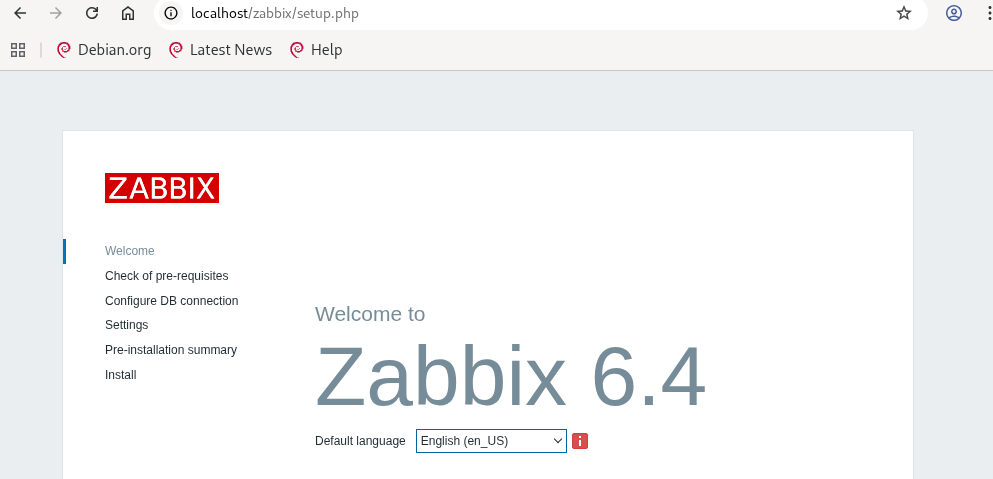
\includegraphics[keepaspectratio,alt={Interface web Zabbix accessible}]{images/zabbix_web_interface.png}}
\emph{Figure 9 --- Interface web Zabbix accessible à
\texttt{http://192.168.1.100/zabbix}}

\subsection{Installation et configuration du serveur
Linux}\label{installation-et-configuration-du-serveur-linux}

\subsubsection{Prérequis}\label{pruxe9requis}

{\def\LTcaptype{none} % do not increment counter
\begin{longtable}[]{@{}ll@{}}
\toprule\noalign{}
Paramètre & Valeur \\
\midrule\noalign{}
\endhead
\bottomrule\noalign{}
\endlastfoot
OS & Debian GNU/Linux 12 (Bookworm) \\
RAM & 2 Go \\
Stockage & 20 Go \\
Adresse IP & 192.168.1.10 (statique via systemd-networkd) \\
Passerelle & 192.168.1.1 \\
\end{longtable}
}

\subsubsection{Configuration de l'adresse IP
statique}\label{configuration-de-ladresse-ip-statique}

\begin{Shaded}
\begin{Highlighting}[]
\CommentTok{\# /etc/systemd/network/10{-}static.network}
\ExtensionTok{[Match]}
\VariableTok{Name}\OperatorTok{=}\NormalTok{enp0s8}

\ExtensionTok{[Network]}
\VariableTok{Address}\OperatorTok{=}\NormalTok{192.168.1.10/24}
\VariableTok{Gateway}\OperatorTok{=}\NormalTok{192.168.1.1}
\VariableTok{DNS}\OperatorTok{=}\NormalTok{8.8.8.8}
\end{Highlighting}
\end{Shaded}

\begin{Shaded}
\begin{Highlighting}[]
\FunctionTok{sudo}\NormalTok{ systemctl restart systemd{-}networkd}
\ExtensionTok{ip}\NormalTok{ addr show enp0s8}
\end{Highlighting}
\end{Shaded}

\subsubsection{Installation de Nginx (serveur web port
80)}\label{installation-de-nginx-serveur-web-port-80}

\begin{Shaded}
\begin{Highlighting}[]
\FunctionTok{sudo}\NormalTok{ apt update}
\FunctionTok{sudo}\NormalTok{ apt install }\AttributeTok{{-}y}\NormalTok{ nginx}
\FunctionTok{sudo}\NormalTok{ systemctl start nginx}
\FunctionTok{sudo}\NormalTok{ systemctl enable nginx}
\FunctionTok{sudo}\NormalTok{ ss }\AttributeTok{{-}tlnp} \KeywordTok{|} \FunctionTok{grep}\NormalTok{ :80}
\end{Highlighting}
\end{Shaded}

\pandocbounded{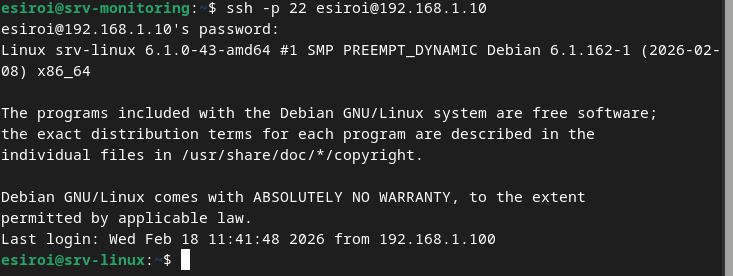
\includegraphics[keepaspectratio,alt={Accès SSH depuis srv-monitoring vers srv-linux}]{images/ssh_acces_from_srv_monitoring_to_srv_linux.png}}
\emph{Figure 10 --- Accès SSH depuis srv-monitoring vers srv-linux}

\subsubsection{Installation de l'agent
Zabbix}\label{installation-de-lagent-zabbix}

\begin{Shaded}
\begin{Highlighting}[]
\FunctionTok{wget}\NormalTok{ https://repo.zabbix.com/zabbix/6.4/debian/pool/main/z/zabbix{-}release/zabbix{-}release\_6.4{-}1+debian12\_all.deb}
\FunctionTok{sudo}\NormalTok{ dpkg }\AttributeTok{{-}i}\NormalTok{ zabbix{-}release\_6.4{-}1+debian12\_all.deb}
\FunctionTok{sudo}\NormalTok{ apt update}
\FunctionTok{sudo}\NormalTok{ apt install }\AttributeTok{{-}y}\NormalTok{ zabbix{-}agent}
\end{Highlighting}
\end{Shaded}

\paragraph{\texorpdfstring{Configuration de
\texttt{/etc/zabbix/zabbix\_agentd.conf}}{Configuration de /etc/zabbix/zabbix\_agentd.conf}}\label{configuration-de-etczabbixzabbix_agentd.conf}

\begin{Shaded}
\begin{Highlighting}[]
\DataTypeTok{Server}\OtherTok{=}\StringTok{192.168.1.100}
\DataTypeTok{ServerActive}\OtherTok{=}\StringTok{192.168.1.100}
\DataTypeTok{Hostname}\OtherTok{=}\StringTok{srv{-}linux}
\end{Highlighting}
\end{Shaded}

\begin{Shaded}
\begin{Highlighting}[]
\FunctionTok{sudo}\NormalTok{ systemctl restart zabbix{-}agent}
\FunctionTok{sudo}\NormalTok{ systemctl enable zabbix{-}agent}
\end{Highlighting}
\end{Shaded}

\pandocbounded{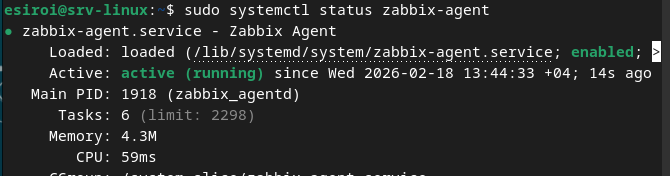
\includegraphics[keepaspectratio,alt={Agent Zabbix actif sur srv-linux}]{images/zabbix_agent_status_on_linux_server.png}}
\emph{Figure 11 --- Agent Zabbix actif sur srv-linux}

\paragraph{Vérification depuis
srv-monitoring}\label{vuxe9rification-depuis-srv-monitoring}

\begin{Shaded}
\begin{Highlighting}[]
\FunctionTok{sudo}\NormalTok{ apt install zabbix{-}get }\AttributeTok{{-}y}
\ExtensionTok{zabbix\_get} \AttributeTok{{-}s}\NormalTok{ 192.168.1.10 }\AttributeTok{{-}k}\NormalTok{ system.hostname}
\CommentTok{\# Résultat : srv{-}linux}
\end{Highlighting}
\end{Shaded}

\pandocbounded{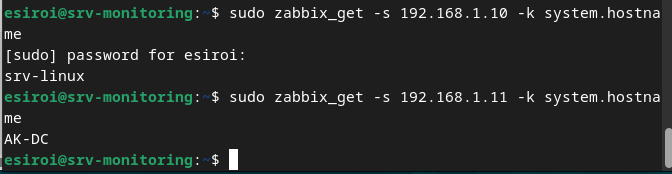
\includegraphics[keepaspectratio,alt={Résultat de zabbix\_get sur srv-linux}]{images/zabbix_get_result.png}}
\emph{Figure 12 --- Résultat de \texttt{zabbix\_get} confirmant la
communication avec l'agent}

\subsubsection{Installation de l'agent
Wazuh}\label{installation-de-lagent-wazuh}

\begin{Shaded}
\begin{Highlighting}[]
\ExtensionTok{curl} \AttributeTok{{-}s}\NormalTok{ https://packages.wazuh.com/key/GPG{-}KEY{-}WAZUH }\KeywordTok{|} \FunctionTok{sudo}\NormalTok{ apt{-}key add }\AttributeTok{{-}}
\BuiltInTok{echo} \StringTok{"deb https://packages.wazuh.com/4.x/apt/ stable main"} \KeywordTok{|} \FunctionTok{sudo}\NormalTok{ tee /etc/apt/sources.list.d/wazuh.list}
\FunctionTok{sudo}\NormalTok{ apt update}
\FunctionTok{sudo}\NormalTok{ apt install }\AttributeTok{{-}y}\NormalTok{ wazuh{-}agent}
\end{Highlighting}
\end{Shaded}

\paragraph{\texorpdfstring{Configuration de
\texttt{/var/ossec/etc/ossec.conf}}{Configuration de /var/ossec/etc/ossec.conf}}\label{configuration-de-varossecetcossec.conf}

\begin{Shaded}
\begin{Highlighting}[]
\NormalTok{\textless{}}\KeywordTok{client}\NormalTok{\textgreater{}}
\NormalTok{  \textless{}}\KeywordTok{server}\NormalTok{\textgreater{}}
\NormalTok{    \textless{}}\KeywordTok{address}\NormalTok{\textgreater{}192.168.1.100\textless{}/}\KeywordTok{address}\NormalTok{\textgreater{}}
\NormalTok{    \textless{}}\KeywordTok{port}\NormalTok{\textgreater{}1514\textless{}/}\KeywordTok{port}\NormalTok{\textgreater{}}
\NormalTok{    \textless{}}\KeywordTok{protocol}\NormalTok{\textgreater{}tcp\textless{}/}\KeywordTok{protocol}\NormalTok{\textgreater{}}
\NormalTok{  \textless{}/}\KeywordTok{server}\NormalTok{\textgreater{}}
\NormalTok{\textless{}/}\KeywordTok{client}\NormalTok{\textgreater{}}
\end{Highlighting}
\end{Shaded}

\begin{Shaded}
\begin{Highlighting}[]
\FunctionTok{sudo}\NormalTok{ systemctl start wazuh{-}agent}
\FunctionTok{sudo}\NormalTok{ systemctl enable wazuh{-}agent}
\FunctionTok{sudo}\NormalTok{ systemctl status wazuh{-}agent}
\end{Highlighting}
\end{Shaded}

\pandocbounded{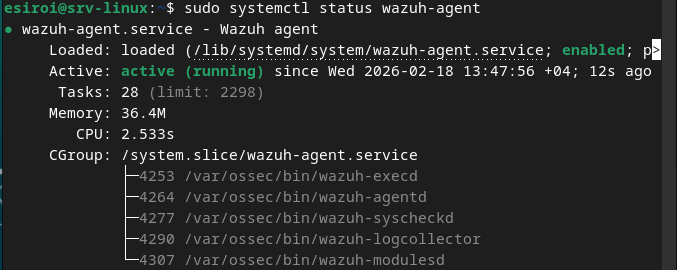
\includegraphics[keepaspectratio,alt={Agent Wazuh v4.7.5 actif sur srv-linux}]{images/wazuh_agent_status_on_linux_server.png}}
\emph{Figure 13 --- Agent Wazuh v4.7.5 actif sur srv-linux}

\subsection{Configuration du pare-feu
pfSense}\label{configuration-du-pare-feu-pfsense}

\subsubsection{Prérequis}\label{pruxe9requis-1}

{\def\LTcaptype{none} % do not increment counter
\begin{longtable}[]{@{}ll@{}}
\toprule\noalign{}
Paramètre & Valeur \\
\midrule\noalign{}
\endhead
\bottomrule\noalign{}
\endlastfoot
OS & pfSense 2.7.0-RELEASE (FreeBSD 14.0-CURRENT) \\
RAM & 1 Go \\
Stockage & 12 Go \\
Interface WAN & 192.168.1.1/24 (Bridge) \\
\end{longtable}
}

\subsubsection{Accès à l'interface
web}\label{accuxe8s-uxe0-linterface-web}

L'interface d'administration est accessible via :

\begin{verbatim}
http://192.168.1.1
Utilisateur : admin
Mot de passe : pfsense
\end{verbatim}

\pandocbounded{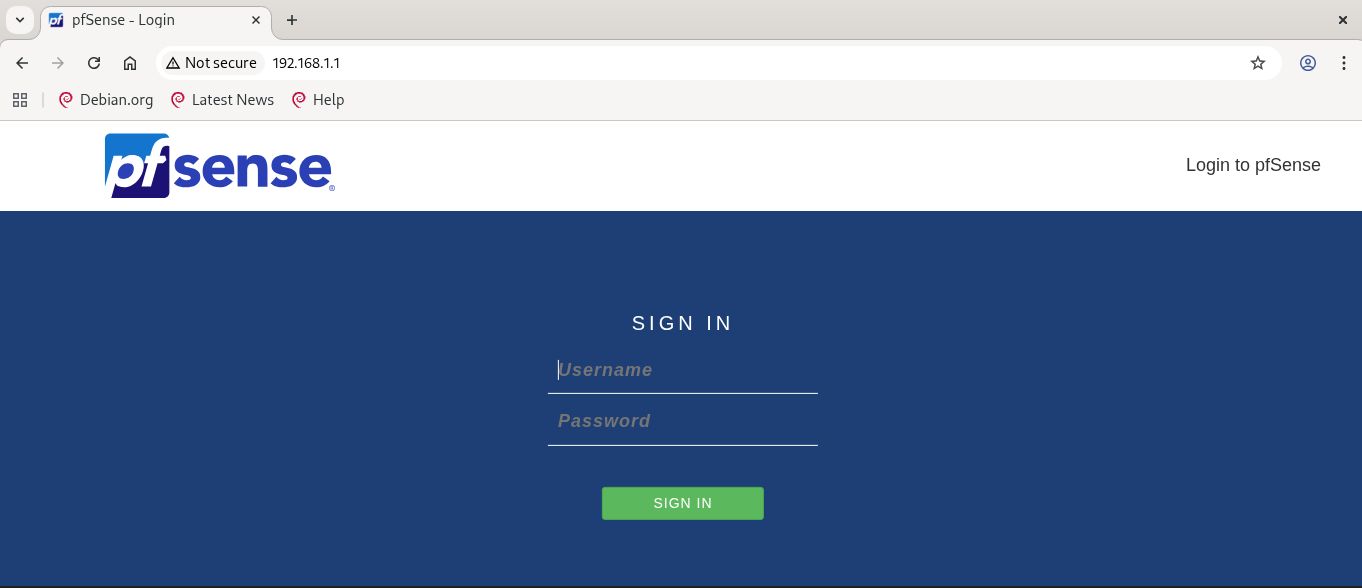
\includegraphics[keepaspectratio,alt={Page de connexion à l'interface web pfSense}]{images/pfsense_web_interface_login.png}}
\emph{Figure 14 --- Page de connexion à l'interface web pfSense}

\pandocbounded{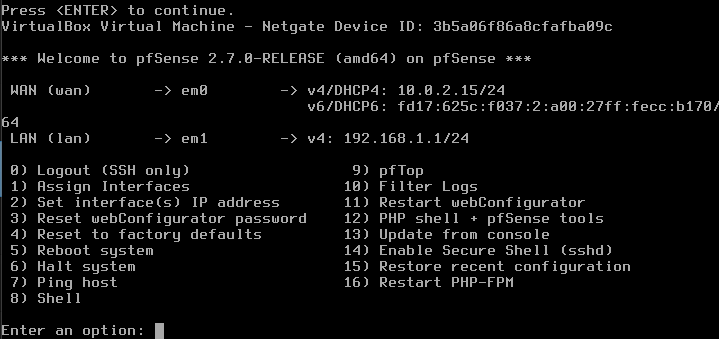
\includegraphics[keepaspectratio,alt={Interface console pfSense}]{images/pfsense_firewall_terminal_interface.png}}
\emph{Figure 15 --- Interface console pfSense (accès terminal)}

\subsubsection{Configuration SNMP}\label{configuration-snmp}

Voir section 2.3.

\subsubsection{Configuration du transfert de logs vers Wazuh
(Syslog)}\label{configuration-du-transfert-de-logs-vers-wazuh-syslog}

Depuis l'interface web pfSense :

\begin{enumerate}
\def\labelenumi{\arabic{enumi}.}
\tightlist
\item
  \textbf{Status → System Logs → Settings}
\item
  Activer \textbf{Send log messages to remote syslog server}
\item
  Configurer :

  \begin{itemize}
  \tightlist
  \item
    \textbf{IP address :} 192.168.1.100
  \item
    \textbf{Port :} 514
  \item
    \textbf{Protocol :} UDP
  \item
    \textbf{Remote Syslog Contents :} System Events, Firewall Events
  \end{itemize}
\end{enumerate}

\pandocbounded{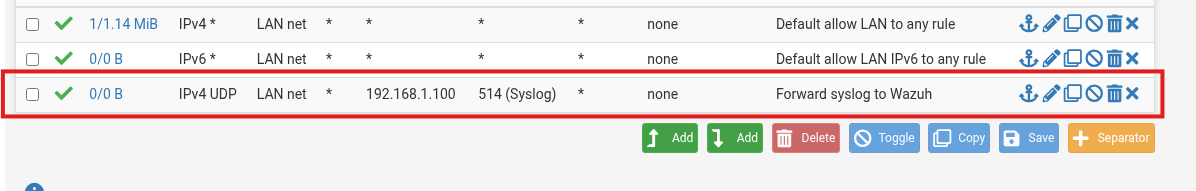
\includegraphics[keepaspectratio,alt={Règle de pare-feu autorisant le syslog vers srv-monitoring}]{images/firewall_rule_for_syslog.png}}
\emph{Figure 16 --- Règle de pare-feu autorisant le transfert syslog
UDP/514 vers srv-monitoring}

\subsection{Configuration du serveur
Windows}\label{configuration-du-serveur-windows}

\subsubsection{Prérequis}\label{pruxe9requis-2}

{\def\LTcaptype{none} % do not increment counter
\begin{longtable}[]{@{}ll@{}}
\toprule\noalign{}
Paramètre & Valeur \\
\midrule\noalign{}
\endhead
\bottomrule\noalign{}
\endlastfoot
OS & Windows Server 2019 (version 10.0.17763) \\
Nom d'hôte & AK-DC \\
RAM & 4 Go \\
Stockage & 60 Go \\
Adresse IP & 192.168.1.11 (statique) \\
Rôle & Active Directory Domain Controller \\
\end{longtable}
}

\subsubsection{Installation de l'agent
Zabbix}\label{installation-de-lagent-zabbix-1}

L'agent Zabbix 6.4 pour Windows a été téléchargé depuis le site officiel
et installé via l'installateur MSI.

\textbf{Configuration dans \texttt{zabbix\_agentd.conf} :}

\begin{Shaded}
\begin{Highlighting}[]
\DataTypeTok{Server}\OtherTok{=}\StringTok{192.168.1.100}
\DataTypeTok{ServerActive}\OtherTok{=}\StringTok{192.168.1.100}
\DataTypeTok{Hostname}\OtherTok{=}\StringTok{AK{-}DC}
\end{Highlighting}
\end{Shaded}

\textbf{Démarrage du service :}

\begin{Shaded}
\begin{Highlighting}[]
\FunctionTok{Start{-}Service} \StringTok{"Zabbix Agent"}
\FunctionTok{Get{-}Service} \OperatorTok{{-}}\NormalTok{Name }\StringTok{"*zabbix*"}
\end{Highlighting}
\end{Shaded}

\textbf{Vérification depuis srv-monitoring :}

\begin{Shaded}
\begin{Highlighting}[]
\ExtensionTok{zabbix\_get} \AttributeTok{{-}s}\NormalTok{ AK{-}DC }\AttributeTok{{-}k}\NormalTok{ system.hostname}
\CommentTok{\# Résultat : AK{-}DC}

\ExtensionTok{zabbix\_get} \AttributeTok{{-}s}\NormalTok{ AK{-}DC }\AttributeTok{{-}k}\NormalTok{ agent.version}
\CommentTok{\# Résultat : 6.4.0}

\ExtensionTok{zabbix\_get} \AttributeTok{{-}s}\NormalTok{ AK{-}DC }\AttributeTok{{-}k}\NormalTok{ agent.ping}
\CommentTok{\# Résultat : 1}
\end{Highlighting}
\end{Shaded}

\subsubsection{Installation de l'agent
Wazuh}\label{installation-de-lagent-wazuh-1}

L'agent Wazuh 4.7.5 pour Windows a été installé via le fichier MSI :

\begin{Shaded}
\begin{Highlighting}[]
\NormalTok{msiexec }\OperatorTok{/}\NormalTok{i }\StringTok{"}\VariableTok{$env}\OperatorTok{:}\VariableTok{TEMP}\StringTok{\textbackslash{}wazuh{-}agent.msi"} \OperatorTok{/}\NormalTok{q WAZUH\_MANAGER}\OperatorTok{=}\StringTok{"192.168.1.100"}\NormalTok{ WAZUH\_REGISTRATION\_SERVER}\OperatorTok{=}\StringTok{"192.168.1.100"}\NormalTok{ PROTOCOL}\OperatorTok{=}\NormalTok{tcp}
\end{Highlighting}
\end{Shaded}

\textbf{Emplacement de l'installation :}
\texttt{C:\textbackslash{}Program\ Files\ (x86)\textbackslash{}ossec-agent\textbackslash{}}

\textbf{Fichier de configuration :}
\texttt{C:\textbackslash{}Program\ Files\ (x86)\textbackslash{}ossec-agent\textbackslash{}ossec.conf}

\begin{Shaded}
\begin{Highlighting}[]
\NormalTok{\textless{}}\KeywordTok{client}\NormalTok{\textgreater{}}
\NormalTok{  \textless{}}\KeywordTok{server}\NormalTok{\textgreater{}}
\NormalTok{    \textless{}}\KeywordTok{address}\NormalTok{\textgreater{}192.168.1.100\textless{}/}\KeywordTok{address}\NormalTok{\textgreater{}}
\NormalTok{    \textless{}}\KeywordTok{manager\_address}\NormalTok{\textgreater{}192.168.1.100\textless{}/}\KeywordTok{manager\_address}\NormalTok{\textgreater{}}
\NormalTok{  \textless{}/}\KeywordTok{server}\NormalTok{\textgreater{}}
\NormalTok{\textless{}/}\KeywordTok{client}\NormalTok{\textgreater{}}
\end{Highlighting}
\end{Shaded}

\textbf{Démarrage du service :}

\begin{Shaded}
\begin{Highlighting}[]
\FunctionTok{Start{-}Service} \OperatorTok{{-}}\NormalTok{Name }\StringTok{"WazuhSvc"}
\FunctionTok{Get{-}Service} \OperatorTok{{-}}\NormalTok{Name }\StringTok{"WazuhSvc"}
\CommentTok{\# Status: Running}
\end{Highlighting}
\end{Shaded}

\textbf{Vérification des logs de l'agent :}

\begin{Shaded}
\begin{Highlighting}[]
\FunctionTok{Get{-}Content} \StringTok{"C:\textbackslash{}Program Files (x86)\textbackslash{}ossec{-}agent\textbackslash{}ossec.log"} \OperatorTok{{-}}\NormalTok{Tail }\DecValTok{20}
\CommentTok{\# 2026/02/19 01:35:32 wazuh{-}agent: INFO: Started (pid: 3032).}
\CommentTok{\# 2026/02/19 01:35:32 wazuh{-}modulesd:syscollector: INFO: Module started.}
\end{Highlighting}
\end{Shaded}

\subsection{Supervision avec Zabbix}\label{supervision-avec-zabbix}

\subsubsection{Ajout des hôtes dans
Zabbix}\label{ajout-des-huxf4tes-dans-zabbix}

Depuis l'interface web \texttt{http://192.168.1.100/zabbix}
(Configuration → Hôtes → Créer un hôte) :

{\def\LTcaptype{none} % do not increment counter
\begin{longtable}[]{@{}
  >{\raggedright\arraybackslash}p{(\linewidth - 8\tabcolsep) * \real{0.2000}}
  >{\raggedright\arraybackslash}p{(\linewidth - 8\tabcolsep) * \real{0.2000}}
  >{\raggedright\arraybackslash}p{(\linewidth - 8\tabcolsep) * \real{0.2000}}
  >{\raggedright\arraybackslash}p{(\linewidth - 8\tabcolsep) * \real{0.2000}}
  >{\raggedright\arraybackslash}p{(\linewidth - 8\tabcolsep) * \real{0.2000}}@{}}
\toprule\noalign{}
\begin{minipage}[b]{\linewidth}\raggedright
Nom d'hôte
\end{minipage} & \begin{minipage}[b]{\linewidth}\raggedright
Interface
\end{minipage} & \begin{minipage}[b]{\linewidth}\raggedright
Type
\end{minipage} & \begin{minipage}[b]{\linewidth}\raggedright
Port
\end{minipage} & \begin{minipage}[b]{\linewidth}\raggedright
Template
\end{minipage} \\
\midrule\noalign{}
\endhead
\bottomrule\noalign{}
\endlastfoot
srv-linux & 192.168.1.10 & Agent Zabbix & 10050 & Linux by Zabbix
agent \\
AK-DC & 192.168.1.11 & Agent Zabbix & 10050 & Windows by Zabbix agent \\
Firewall & 192.168.1.1 & SNMPv2c & 161 & Generic SNMP / pfSense by
SNMP \\
\end{longtable}
}

\textbf{Macro SNMP pour le firewall :}

\begin{verbatim}
{$SNMP_COMMUNITY} = public
\end{verbatim}

\pandocbounded{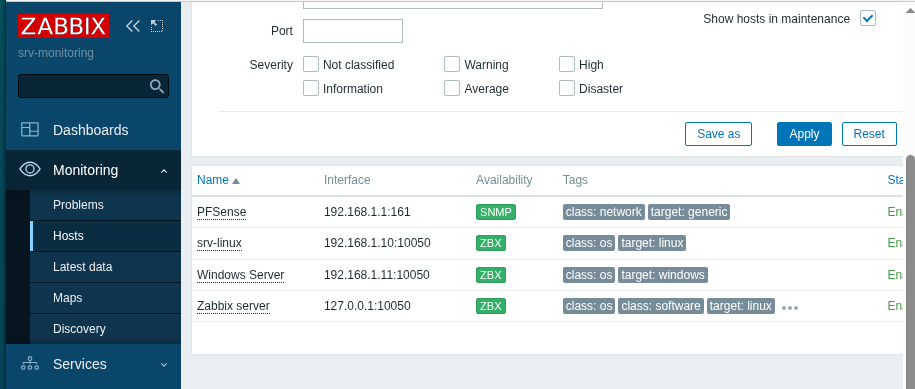
\includegraphics[keepaspectratio,alt={Les 3 hôtes supervisés dans le tableau de bord Zabbix}]{images/zabbix_3_hosts_supervised.png}}
\emph{Figure 17 --- Les 3 hôtes supervisés dans Zabbix : srv-linux,
AK-DC et firewall}

\subsubsection{Vérification de la
connectivité}\label{vuxe9rification-de-la-connectivituxe9}

\begin{Shaded}
\begin{Highlighting}[]
\CommentTok{\# Depuis srv{-}monitoring}
\ExtensionTok{zabbix\_get} \AttributeTok{{-}s}\NormalTok{ 192.168.1.10 }\AttributeTok{{-}k}\NormalTok{ system.hostname   }\CommentTok{\# → srv{-}linux}
\ExtensionTok{zabbix\_get} \AttributeTok{{-}s}\NormalTok{ AK{-}DC }\AttributeTok{{-}k}\NormalTok{ agent.ping               }\CommentTok{\# → 1}
\ExtensionTok{zabbix\_get} \AttributeTok{{-}s}\NormalTok{ AK{-}DC }\AttributeTok{{-}k}\NormalTok{ agent.version            }\CommentTok{\# → 6.4.0}
\ExtensionTok{snmpwalk} \AttributeTok{{-}v}\NormalTok{ 2c }\AttributeTok{{-}c}\NormalTok{ public 192.168.1.1             }\CommentTok{\# → pfSense info}
\ExtensionTok{snmpwalk} \AttributeTok{{-}v}\NormalTok{ 2c }\AttributeTok{{-}c}\NormalTok{ public 192.168.1.10            }\CommentTok{\# → Linux srv{-}linux info}
\end{Highlighting}
\end{Shaded}

\subsubsection{Supervision SNMP avancée du
firewall}\label{supervision-snmp-avancuxe9e-du-firewall}

Un item SNMP a été configuré pour surveiller le trafic de l'interface
WAN du firewall :

\begin{itemize}
\tightlist
\item
  \textbf{Nom :} Interface WAN traffic
\item
  \textbf{Type :} SNMP v2c
\item
  \textbf{OID :} \texttt{.1.3.6.1.2.1.2.2.1.10.1} (octets entrants)
\item
  \textbf{Unité :} B
\item
  \textbf{Intervalle :} 60s
\end{itemize}

\pandocbounded{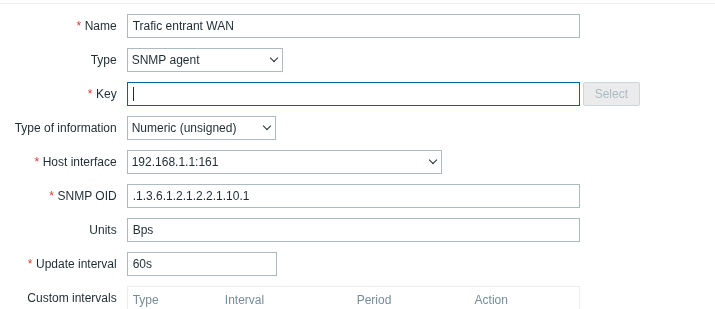
\includegraphics[keepaspectratio,alt={Configuration de l'item SNMP pour l'interface WAN}]{images/item_config_for_snmp_wan_interface.png}}
\emph{Figure 18 --- Configuration de l'item SNMP pour surveiller le
trafic de l'interface WAN}

\pandocbounded{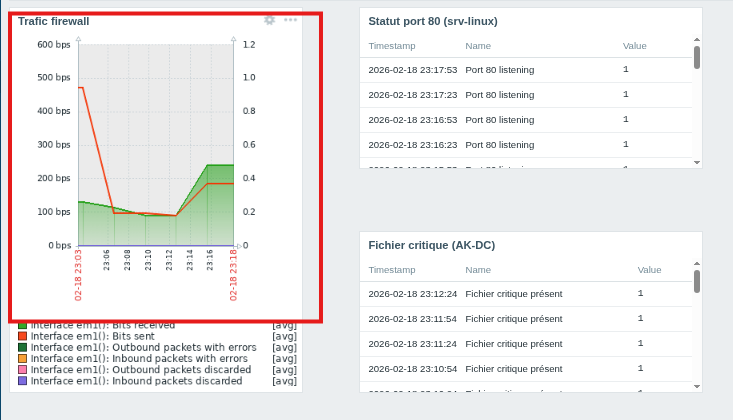
\includegraphics[keepaspectratio,alt={Trafic réseau visible dans Zabbix après un flood ping}]{images/network_trafic_after_flood_ping.png}}
\emph{Figure 19 --- Trafic réseau visible dans Zabbix après un flood
ping sur l'interface WAN}

\subsection{Supervision avancée --- Sondes et
alertes}\label{supervision-avancuxe9e-sondes-et-alertes}

\subsubsection{Supervision du port 80
(srv-linux)}\label{supervision-du-port-80-srv-linux}

\paragraph{Objectif}\label{objectif}

Détecter en temps réel si le service web Nginx est arrêté sur srv-linux
et lever une alerte.

\paragraph{Création de l'item}\label{cruxe9ation-de-litem}

Dans \textbf{Configuration → Hôtes → srv-linux → Items → Create item} :

{\def\LTcaptype{none} % do not increment counter
\begin{longtable}[]{@{}ll@{}}
\toprule\noalign{}
Paramètre & Valeur \\
\midrule\noalign{}
\endhead
\bottomrule\noalign{}
\endlastfoot
Nom & Port 80 listening \\
Type & Zabbix agent \\
Clé & \texttt{net.tcp.listen{[}80{]}} \\
Type d'information & Numeric (unsigned) \\
Intervalle & 30s \\
\end{longtable}
}

La clé \texttt{net.tcp.listen{[}80{]}} retourne \texttt{1} si le port
est en écoute, \texttt{0} sinon.

\paragraph{Création du trigger}\label{cruxe9ation-du-trigger}

{\def\LTcaptype{none} % do not increment counter
\begin{longtable}[]{@{}ll@{}}
\toprule\noalign{}
Paramètre & Valeur \\
\midrule\noalign{}
\endhead
\bottomrule\noalign{}
\endlastfoot
Nom & Port 80 is down on srv-linux \\
Sévérité & High \\
Expression & \texttt{last(/srv-linux/net.tcp.listen{[}80{]})=0} \\
\end{longtable}
}

\pandocbounded{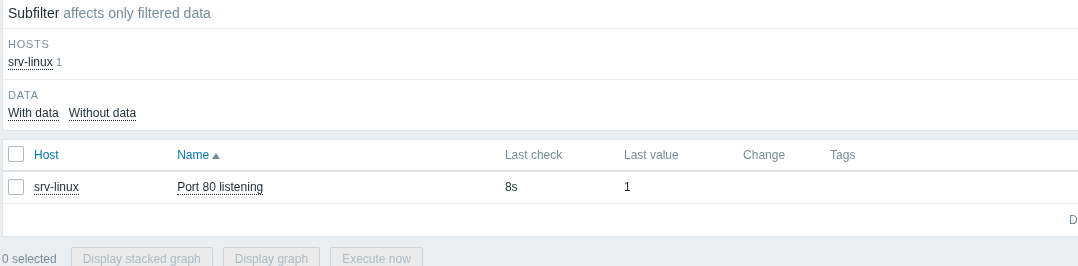
\includegraphics[keepaspectratio,alt={Valeur de l'item port 80 dans Latest data}]{images/port_80_litening_in_latest_data.png}}
\emph{Figure 20 --- Valeur de l'item \texttt{net.tcp.listen{[}80{]}}
visible dans ``Latest data'' (valeur = 1, port actif)}

\pandocbounded{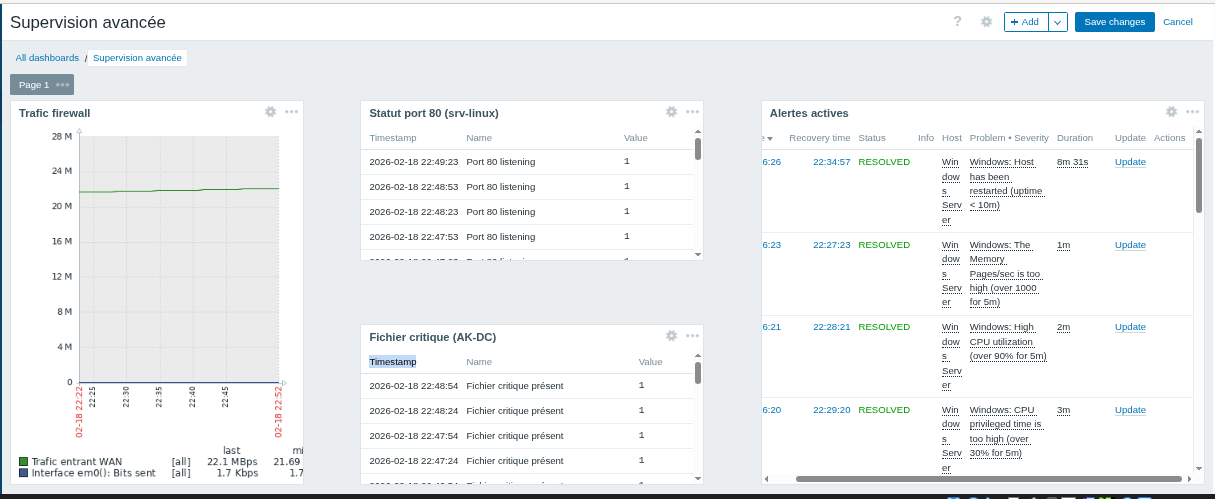
\includegraphics[keepaspectratio,alt={Dashboard Zabbix avant la simulation}]{images/sup_avance_dashboard_before_simulation.png}}
\emph{Figure 21 --- Dashboard Zabbix avant la simulation --- aucune
alerte active}

\paragraph{Simulation de l'arrêt du
service}\label{simulation-de-larruxeat-du-service}

\begin{Shaded}
\begin{Highlighting}[]
\CommentTok{\# Sur srv{-}linux}
\FunctionTok{sudo}\NormalTok{ systemctl stop nginx}
\end{Highlighting}
\end{Shaded}

\pandocbounded{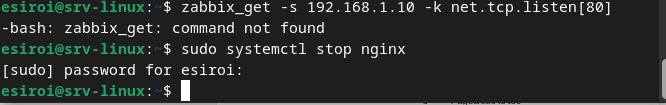
\includegraphics[keepaspectratio,alt={Arrêt du service Nginx sur srv-linux}]{images/simulation_nginx_stop.png}}
\emph{Figure 22 --- Arrêt du service Nginx via
\texttt{systemctl\ stop\ nginx}}

\pandocbounded{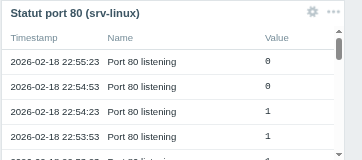
\includegraphics[keepaspectratio,alt={Alerte déclenchée dans Zabbix --- port 80 passe à 0}]{images/simulation_status_port_80_0.png}}
\emph{Figure 23 --- Alerte déclenchée dans Zabbix : l'item passe à 0, le
trigger se déclenche}

\begin{Shaded}
\begin{Highlighting}[]
\CommentTok{\# Redémarrage}
\FunctionTok{sudo}\NormalTok{ systemctl start nginx}
\end{Highlighting}
\end{Shaded}

\subsubsection{Supervision de la présence d'un fichier critique
(AK-DC/Windows)}\label{supervision-de-la-pruxe9sence-dun-fichier-critique-ak-dcwindows}

\paragraph{Objectif}\label{objectif-1}

Détecter la suppression d'un fichier critique sur le contrôleur de
domaine Windows et envoyer une alerte.

\paragraph{Création du fichier
surveillé}\label{cruxe9ation-du-fichier-surveilluxe9}

Sur AK-DC (PowerShell, en admin) :

\begin{Shaded}
\begin{Highlighting}[]
\FunctionTok{New{-}Item} \OperatorTok{{-}}\NormalTok{ItemType Directory }\OperatorTok{{-}}\NormalTok{Path }\StringTok{"C:\textbackslash{}Supervision\textbackslash{}"} \OperatorTok{{-}}\NormalTok{Force}
\FunctionTok{New{-}Item} \OperatorTok{{-}}\NormalTok{ItemType File }\OperatorTok{{-}}\NormalTok{Path }\StringTok{"C:\textbackslash{}Supervision\textbackslash{}fichier\_critique.txt"}\NormalTok{ \textasciigrave{}}
    \OperatorTok{{-}}\NormalTok{Value }\StringTok{"Fichier de supervision ESIROI {-} NE PAS SUPPRIMER"}
\end{Highlighting}
\end{Shaded}

\paragraph{Configuration de l'agent Zabbix
(UserParameter)}\label{configuration-de-lagent-zabbix-userparameter}

Dans
\texttt{C:\textbackslash{}Program\ Files\textbackslash{}Zabbix\ Agent\textbackslash{}zabbix\_agentd.conf}
:

\begin{Shaded}
\begin{Highlighting}[]
\DataTypeTok{UserParameter}\OtherTok{=}\StringTok{check.file.exists[*],powershell {-}Command "if (Test{-}Path {-}Path \textquotesingle{}$1\textquotesingle{}) \{ echo 1 \} else \{ echo 0 \}"}
\end{Highlighting}
\end{Shaded}

Redémarrer le service après modification :

\begin{Shaded}
\begin{Highlighting}[]
\FunctionTok{Restart{-}Service} \StringTok{"Zabbix Agent"}
\end{Highlighting}
\end{Shaded}

\paragraph{Création de l'item}\label{cruxe9ation-de-litem-1}

{\def\LTcaptype{none} % do not increment counter
\begin{longtable}[]{@{}ll@{}}
\toprule\noalign{}
Paramètre & Valeur \\
\midrule\noalign{}
\endhead
\bottomrule\noalign{}
\endlastfoot
Nom & Fichier critique présent \\
Type & Zabbix agent \\
Clé &
\texttt{vfs.file.exists{[}C:\textbackslash{}Supervision\textbackslash{}fichier\_critique.txt{]}} \\
Type d'information & Numeric (unsigned) \\
Intervalle & 30s \\
\end{longtable}
}

\paragraph{Création du trigger}\label{cruxe9ation-du-trigger-1}

{\def\LTcaptype{none} % do not increment counter
\begin{longtable}[]{@{}
  >{\raggedright\arraybackslash}p{(\linewidth - 2\tabcolsep) * \real{0.5000}}
  >{\raggedright\arraybackslash}p{(\linewidth - 2\tabcolsep) * \real{0.5000}}@{}}
\toprule\noalign{}
\begin{minipage}[b]{\linewidth}\raggedright
Paramètre
\end{minipage} & \begin{minipage}[b]{\linewidth}\raggedright
Valeur
\end{minipage} \\
\midrule\noalign{}
\endhead
\bottomrule\noalign{}
\endlastfoot
Nom & Fichier critique absent sur AK-DC \\
Sévérité & High \\
Expression &
\texttt{last(/AK-DC/vfs.file.exists{[}C:\textbackslash{}Supervision\textbackslash{}fichier\_critique.txt{]})=0} \\
\end{longtable}
}

\pandocbounded{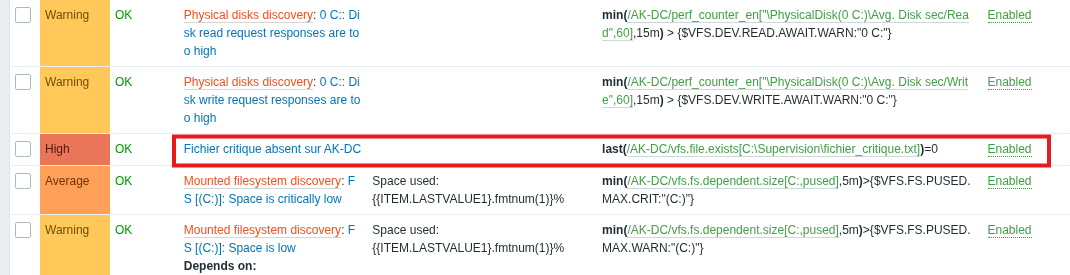
\includegraphics[keepaspectratio,alt={Règle de trigger pour la surveillance du fichier critique}]{images/trigger_rules_critic_files.png}}
\emph{Figure 24 --- Règle de trigger configurée pour détecter l'absence
du fichier critique}

\paragraph{Test et simulation}\label{test-et-simulation}

\begin{Shaded}
\begin{Highlighting}[]
\CommentTok{\# Simuler la suppression}
\FunctionTok{Remove{-}Item}\NormalTok{ C}\OperatorTok{:}\NormalTok{\textbackslash{}Supervision\textbackslash{}fichier\_critique}\OperatorTok{.}\FunctionTok{txt} \OperatorTok{{-}}\NormalTok{Force}
\end{Highlighting}
\end{Shaded}

\pandocbounded{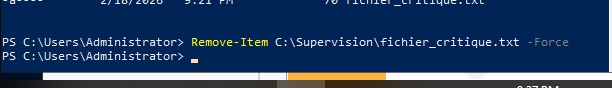
\includegraphics[keepaspectratio,alt={Fichier critique supprimé sur AK-DC}]{images/critic_file_removed.png}}
\emph{Figure 25 --- Suppression du fichier critique
\texttt{C:\textbackslash{}Supervision\textbackslash{}fichier\_critique.txt}}

\pandocbounded{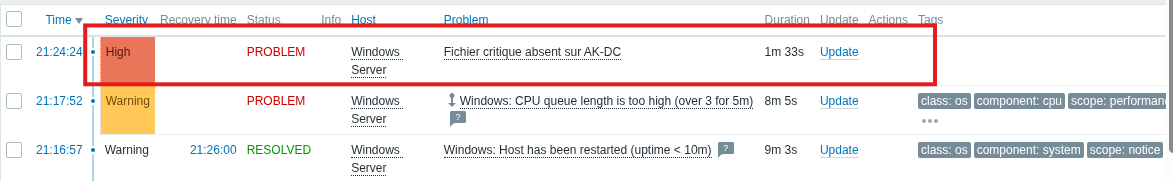
\includegraphics[keepaspectratio,alt={Alerte déclenchée dans Zabbix après suppression du fichier}]{images/alert_result_critic_file_removed.png}}
\emph{Figure 26 --- Alerte de niveau ``High'' déclenchée dans Zabbix
après la suppression}

\pandocbounded{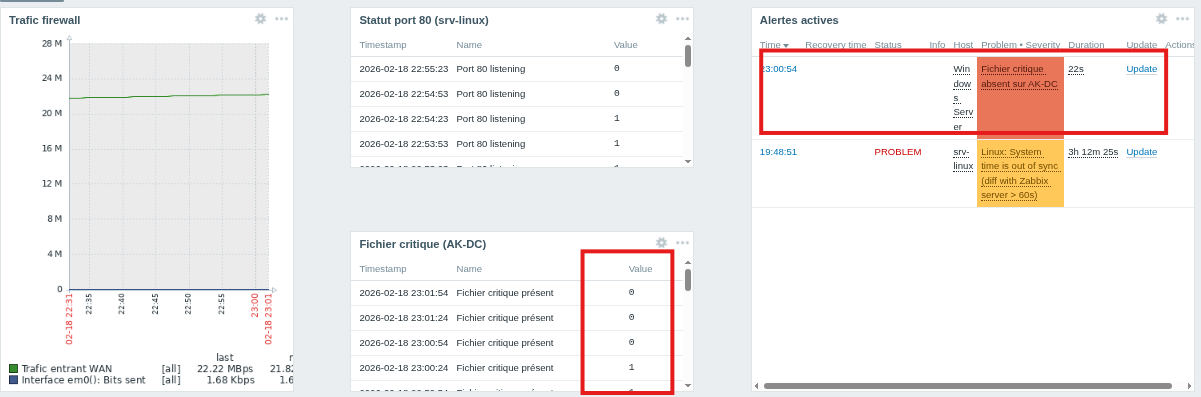
\includegraphics[keepaspectratio,alt={Dashboard Wazuh après suppression du fichier}]{images/dashboard_after_critic_file_deleted.png}}
\emph{Figure 27 --- Dashboard après suppression du fichier critique :
alerte active visible}

\begin{Shaded}
\begin{Highlighting}[]
\CommentTok{\# Recréer le fichier}
\FunctionTok{New{-}Item} \OperatorTok{{-}}\NormalTok{ItemType File }\OperatorTok{{-}}\NormalTok{Path }\StringTok{"C:\textbackslash{}Supervision\textbackslash{}fichier\_critique.txt"} \OperatorTok{{-}}\NormalTok{Value }\StringTok{"Présent"}
\end{Highlighting}
\end{Shaded}

\pandocbounded{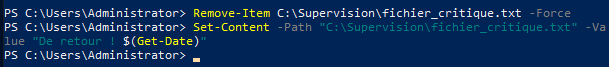
\includegraphics[keepaspectratio,alt={Fichier critique recréé sur AK-DC}]{images/critic_file_recreated.png}}
\emph{Figure 28 --- Recréation du fichier critique sur AK-DC}

\pandocbounded{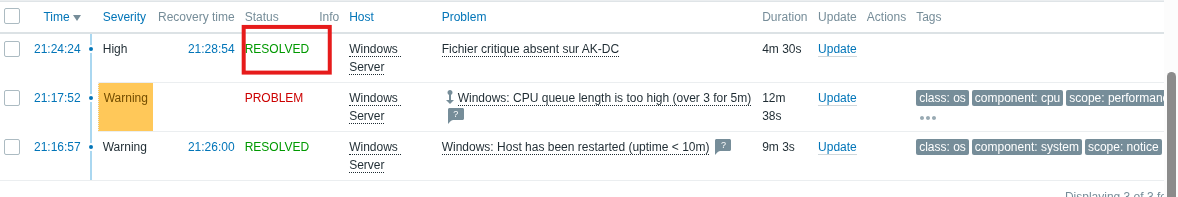
\includegraphics[keepaspectratio,alt={Alerte résolue après recréation du fichier}]{images/alert_resolved_after_critic_file_back.png}}
\emph{Figure 29 --- Alerte résolue automatiquement après recréation du
fichier}

\subsection{SIEM Wazuh --- Centralisation des
logs}\label{siem-wazuh-centralisation-des-logs}

\subsubsection{Architecture Wazuh
All-in-One}\label{architecture-wazuh-all-in-one}

Wazuh a été déployé en mode All-in-One sur \texttt{srv-monitoring}
(192.168.1.100), ce qui regroupe sur une seule machine les trois
composants :

\begin{itemize}
\tightlist
\item
  \textbf{Wazuh Manager} : collecte et analyse des événements de
  sécurité
\item
  \textbf{Wazuh Indexer} : indexation et stockage des données (basé sur
  OpenSearch)
\item
  \textbf{Wazuh Dashboard} : interface web de visualisation
\end{itemize}

\subsubsection{Installation Wazuh
(All-in-One)}\label{installation-wazuh-all-in-one}

\begin{Shaded}
\begin{Highlighting}[]
\ExtensionTok{curl} \AttributeTok{{-}sO}\NormalTok{ https://packages.wazuh.com/4.7/wazuh{-}install.sh}
\FunctionTok{chmod}\NormalTok{ +x wazuh{-}install.sh}
\FunctionTok{sudo}\NormalTok{ ./wazuh{-}install.sh }\AttributeTok{{-}{-}generate{-}config{-}files}
\FunctionTok{sudo}\NormalTok{ ./wazuh{-}install.sh }\AttributeTok{{-}{-}wazuh{-}indexer}\NormalTok{ node{-}1}
\FunctionTok{sudo}\NormalTok{ ./wazuh{-}install.sh }\AttributeTok{{-}{-}start{-}cluster}
\FunctionTok{sudo}\NormalTok{ ./wazuh{-}install.sh }\AttributeTok{{-}{-}wazuh{-}server}\NormalTok{ wazuh{-}1}
\FunctionTok{sudo}\NormalTok{ ./wazuh{-}install.sh }\AttributeTok{{-}{-}wazuh{-}dashboard}\NormalTok{ dashboard}
\end{Highlighting}
\end{Shaded}

\textbf{Récupération du mot de passe admin :}

\begin{Shaded}
\begin{Highlighting}[]
\FunctionTok{sudo}\NormalTok{ tar }\AttributeTok{{-}O} \AttributeTok{{-}xvf}\NormalTok{ wazuh{-}install{-}files.tar wazuh{-}install{-}files/wazuh{-}passwords.txt}
\end{Highlighting}
\end{Shaded}

\textbf{Accès au dashboard :}

\begin{verbatim}
URL      : https://192.168.1.100
Login    : admin
Password : (récupéré lors de l'installation)
\end{verbatim}

\pandocbounded{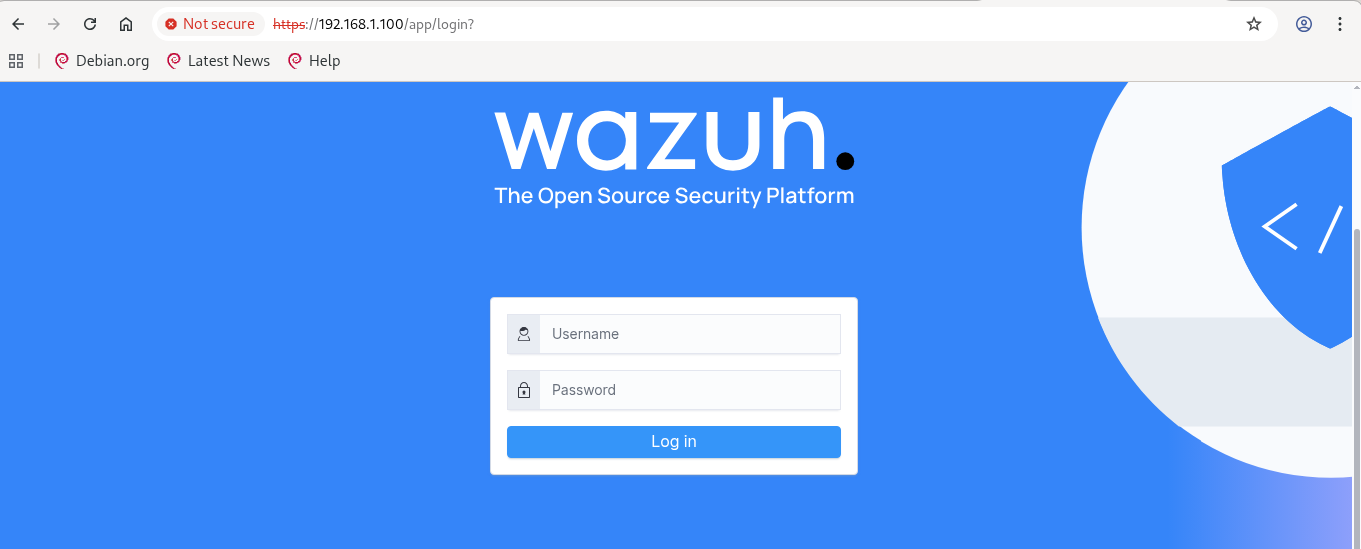
\includegraphics[keepaspectratio,alt={Interface web Wazuh Dashboard}]{images/wazuh_web_interface.png}}
\emph{Figure 30 --- Interface web Wazuh Dashboard accessible à
\texttt{https://192.168.1.100}}

\pandocbounded{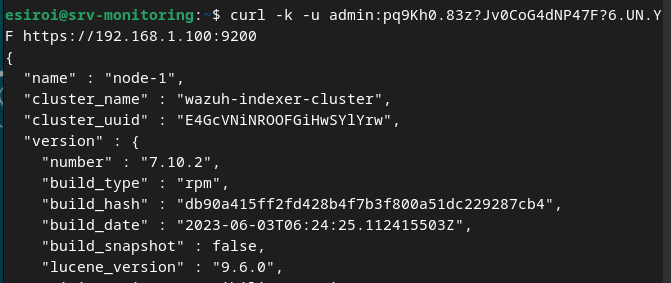
\includegraphics[keepaspectratio,alt={Vérification de l'accès au dashboard Wazuh via curl}]{images/curl_acces_on_wazuh_dashboard.png}}
\emph{Figure 31 --- Vérification de l'accès HTTPS au dashboard Wazuh via
curl}

\pandocbounded{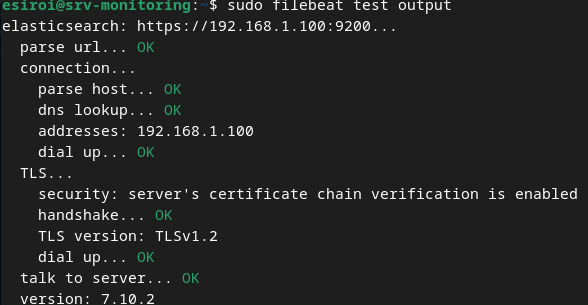
\includegraphics[keepaspectratio,alt={Test de la sortie Filebeat vers l'indexer}]{images/filebeat_output_test.png}}
\emph{Figure 32 --- Test de la sortie Filebeat confirmant la connexion
vers le Wazuh Indexer}

\subsubsection{Agents Wazuh
enregistrés}\label{agents-wazuh-enregistruxe9s}

Après l'installation et la configuration des agents sur srv-linux et
AK-DC :

\pandocbounded{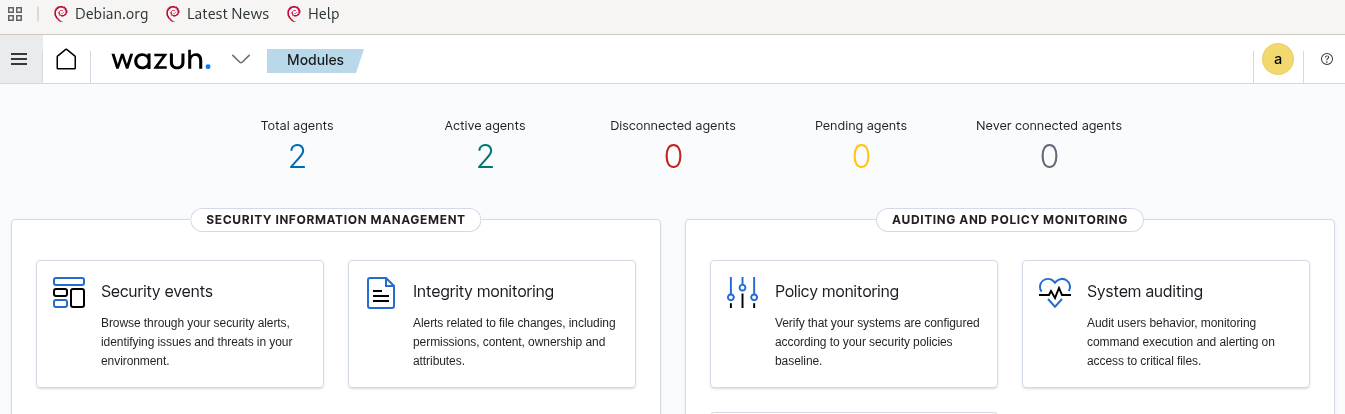
\includegraphics[keepaspectratio,alt={Agents Wazuh visibles dans le dashboard}]{images/wazuh_dashboard_agent_diplayed.png}}
\emph{Figure 33 --- Agents Wazuh affichés dans le dashboard}

\pandocbounded{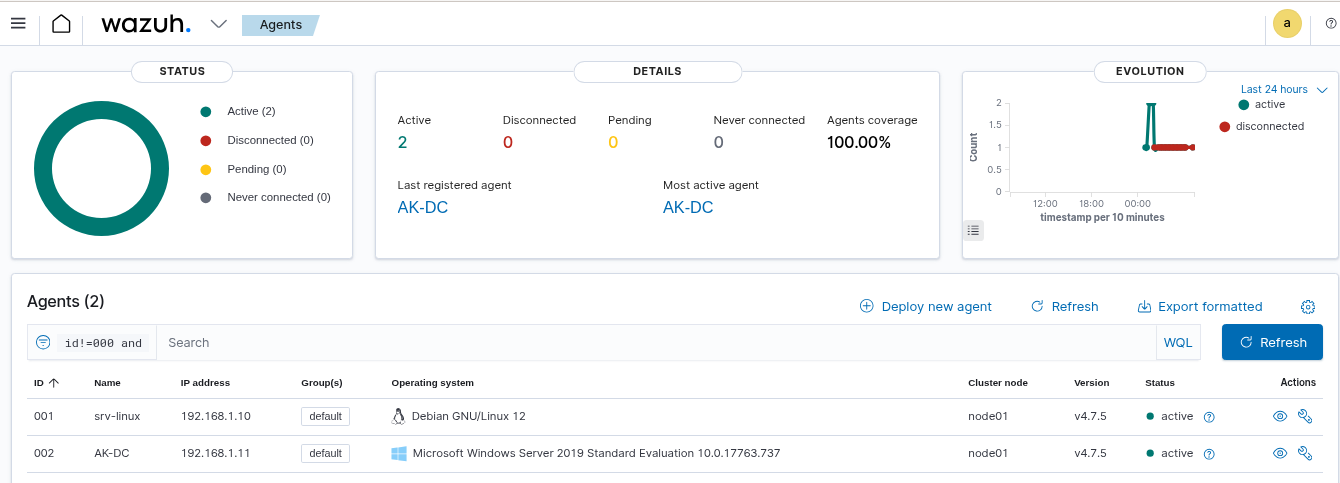
\includegraphics[keepaspectratio,alt={Deux agents actifs dans le tableau de bord Wazuh}]{images/2_agents_on_dashboard.png}}
\emph{Figure 34 --- Deux agents actifs : srv-linux et AK-DC dans le
tableau de bord Wazuh}

\pandocbounded{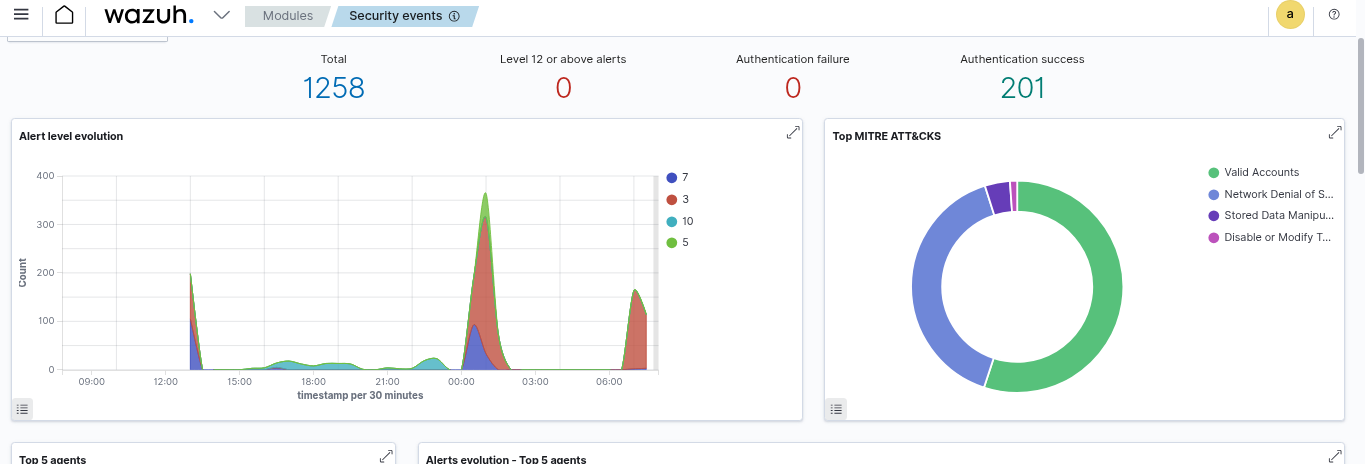
\includegraphics[keepaspectratio,alt={Événements de sécurité remontés par les agents}]{images/agents_securtiy_events.png}}
\emph{Figure 35 --- Événements de sécurité collectés et affichés dans le
dashboard Wazuh}

\subsubsection{Collecte des logs
système}\label{collecte-des-logs-systuxe8me}

Les agents Wazuh collectent automatiquement :

\textbf{Sur srv-linux :} - Logs \texttt{/var/log/auth.log}
(authentification SSH) - Logs système \texttt{/var/log/syslog} -
Surveillance d'intégrité de fichiers (FIM)

\textbf{Sur AK-DC (Windows) :} - Event Channel System
(\texttt{eventchannel}) - Logs d'authentification Windows - Surveillance
Active Directory

Configuration dans \texttt{ossec.conf} (AK-DC) :

\begin{Shaded}
\begin{Highlighting}[]
\NormalTok{\textless{}}\KeywordTok{localfile}\NormalTok{\textgreater{}}
\NormalTok{  \textless{}}\KeywordTok{location}\NormalTok{\textgreater{}System\textless{}/}\KeywordTok{location}\NormalTok{\textgreater{}}
\NormalTok{  \textless{}}\KeywordTok{log\_format}\NormalTok{\textgreater{}eventchannel\textless{}/}\KeywordTok{log\_format}\NormalTok{\textgreater{}}
\NormalTok{\textless{}/}\KeywordTok{localfile}\NormalTok{\textgreater{}}
\end{Highlighting}
\end{Shaded}

\textbf{Depuis pfSense :} - Logs syslog transmis en UDP/514 vers
192.168.1.100

\subsection{Simulation d'une attaque par force brute
SSH}\label{simulation-dune-attaque-par-force-brute-ssh}

\subsubsection{Objectif}\label{objectif-2}

Simuler une attaque par dictionnaire sur le service SSH de srv-linux et
vérifier que Wazuh détecte et corrèle les événements dans le SIEM.

\subsubsection{Préparation de
l'attaque}\label{pruxe9paration-de-lattaque}

\textbf{Depuis srv-monitoring, installation de l'outil d'attaque :}

\begin{Shaded}
\begin{Highlighting}[]
\FunctionTok{sudo}\NormalTok{ apt update}
\FunctionTok{sudo}\NormalTok{ apt install }\AttributeTok{{-}y}\NormalTok{ hydra}
\end{Highlighting}
\end{Shaded}

\textbf{Création d'un dictionnaire de mots de passe :}

\begin{Shaded}
\begin{Highlighting}[]
\FunctionTok{cat} \OperatorTok{\textgreater{}}\NormalTok{ PASSWD\_LIST.txt }\OperatorTok{\textless{}\textless{} EOF}
\StringTok{password}
\StringTok{123456}
\StringTok{admin}
\StringTok{root}
\StringTok{test}
\StringTok{esiroi}
\StringTok{debian}
\StringTok{wrongpass}
\StringTok{badpassword}
\StringTok{motdepasse}
\StringTok{passtest}
\StringTok{lastpass}
\OperatorTok{EOF}
\end{Highlighting}
\end{Shaded}

\subsubsection{Lancement de l'attaque}\label{lancement-de-lattaque}

\begin{Shaded}
\begin{Highlighting}[]
\FunctionTok{sudo}\NormalTok{ hydra }\AttributeTok{{-}l}\NormalTok{ esiroi }\AttributeTok{{-}P}\NormalTok{ PASSWD\_LIST.txt 192.168.1.10 ssh}
\end{Highlighting}
\end{Shaded}

\textbf{Résultat de l'attaque :}

\begin{verbatim}
[DATA] max 13 tasks per 1 server, overall 13 tasks, 13 login tries (l:1/p:13)
[DATA] attacking ssh://192.168.1.10:22/
1 of 1 target completed, 0 valid password found
\end{verbatim}

Hydra n'a pas trouvé le mot de passe correct dans la liste (attendu),
mais les tentatives d'authentification ont bien été enregistrées dans
les logs de srv-linux.

\pandocbounded{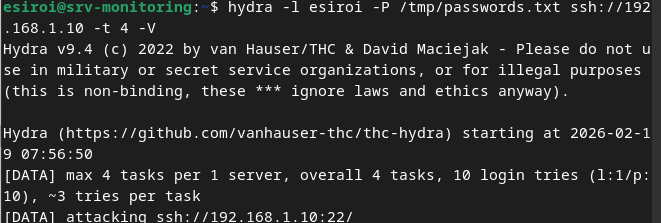
\includegraphics[keepaspectratio,alt={Lancement de l'attaque Hydra depuis srv-monitoring}]{images/simutation_attaque_brute_force.png}}
\emph{Figure 36 --- Lancement de l'attaque par force brute SSH avec
Hydra depuis srv-monitoring}

\subsubsection{Détection par Wazuh}\label{duxe9tection-par-wazuh}

Wazuh a détecté les tentatives de connexion SSH grâce aux règles de
corrélation intégrées (règle 5712 --- SSH brute force).

\pandocbounded{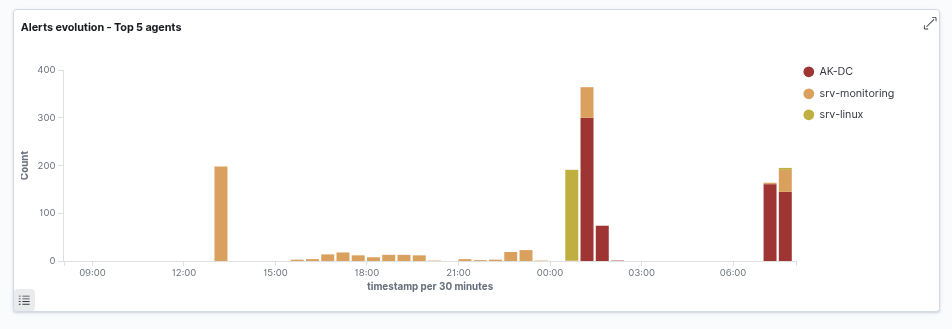
\includegraphics[keepaspectratio,alt={Wazuh --- Top 5 des attaques détectées incluant la force brute SSH}]{images/top_5_attacks_detected_ssh_brute_force.png}}
\emph{Figure 37 --- Wazuh : Top 5 des attaques détectées --- la force
brute SSH apparaît en première position}

\subsubsection{Analyse dans le Dashboard
Wazuh}\label{analyse-dans-le-dashboard-wazuh}

Dans le Dashboard Wazuh → \textbf{Threat Hunting} → \textbf{srv-linux} :

\begin{itemize}
\tightlist
\item
  Augmentation significative des événements ``Authentication Failure''
\item
  Corrélation des tentatives multiples depuis la même source
  (192.168.1.100)
\item
  Classification automatique de l'attaque comme \textbf{brute force SSH}
\item
  Règle MITRE ATT\&CK associée : \textbf{T1110 --- Brute Force}
\end{itemize}

Ce résultat confirme l'efficacité du SIEM pour détecter des attaques en
temps réel, même sans intervention manuelle.

\subsection{Conclusion}\label{conclusion}

Ce travail pratique a permis de déployer et de valider une
infrastructure complète de supervision et de sécurité réseau, intégrant
les outils professionnels Zabbix et Wazuh.

\subsubsection{Bilan des réalisations}\label{bilan-des-ruxe9alisations}

\textbf{Étape 1 --- Infrastructure de base :} - Déploiement de 4
machines virtuelles (srv-monitoring Debian 12, srv-linux Debian 12,
AK-DC Windows Server 2019, pfSense 2.7.0) - Configuration du réseau
\texttt{192.168.1.0/24} en mode Bridge - SNMP configuré et validé sur
srv-linux et pfSense - Zabbix Server 6.4 installé avec MariaDB sur
srv-monitoring - Les 3 hôtes cibles supervisés et visibles dans le
tableau de bord Zabbix

\textbf{Étape 2 --- Supervision avancée :} - Item
\texttt{net.tcp.listen{[}80{]}} configuré sur srv-linux avec déclencheur
et alerte testés - Item \texttt{vfs.file.exists} configuré sur AK-DC
avec simulation de suppression du fichier critique et validation de
l'alerte

\textbf{Étape 3 --- Centralisation des logs :} - Wazuh All-in-One
installé sur srv-monitoring - Agents Wazuh déployés sur srv-linux
(v4.7.5) et AK-DC (v4.7.5) - Logs pfSense transmis via syslog UDP/514 -
Événements de sécurité collectés et indexés dans le Dashboard Wazuh

\textbf{Étape 4 --- Simulation d'attaque :} - Attaque SSH par force
brute simulée avec Hydra depuis srv-monitoring vers srv-linux -
Détection automatique par Wazuh et corrélation des événements dans le
SIEM - Classification MITRE ATT\&CK validée (T1110 --- Brute Force)

\subsubsection{Points techniques
notables}\label{points-techniques-notables}

\begin{itemize}
\tightlist
\item
  La gestion du réseau via \texttt{systemd-networkd} a nécessité de
  désactiver NetworkManager après l'installation de GNOME pour éviter
  les conflits.
\item
  L'agent Wazuh sur Windows Server était installé dans le chemin non
  standard
  \texttt{C:\textbackslash{}Program\ Files\ (x86)\textbackslash{}ossec-agent\textbackslash{}}
  (héritage OSSEC), ce qui a nécessité un diagnostic approfondi.
\item
  Le renommage de l'hôte Windows de \texttt{srv-windows} en
  \texttt{AK-DC} dans Zabbix a résolu les erreurs de correspondance de
  hostname entre l'agent et le serveur.
\end{itemize}

\subsubsection{Perspectives}\label{perspectives}

Cette infrastructure constitue une base solide pour aller plus loin :
mise en place de SNMPv3 (chiffrement et authentification), configuration
d'alertes par email, intégration de tableaux de bord personnalisés
Grafana, et déploiement d'un système de réponse automatique aux
incidents (Active Response Wazuh).

\subsection{Références}\label{ruxe9fuxe9rences}

\begin{enumerate}
\def\labelenumi{\arabic{enumi}.}
\tightlist
\item
  Zabbix SIA, \emph{Documentation officielle Zabbix 6.4},
  https://www.zabbix.com/documentation/6.4/
\item
  Wazuh Inc., \emph{Installation Guide --- All-in-One Deployment},
  https://documentation.wazuh.com/current/installation-guide/
\item
  Wazuh Inc., \emph{Blocking SSH Brute Force Attacks},
  https://documentation.wazuh.com/current/user-manual/capabilities/active-response/
\item
  Netgate, \emph{pfSense Documentation},
  https://docs.netgate.com/pfsense/en/latest/
\item
  Debian Project, \emph{Debian GNU/Linux 12 Administrator's Handbook},
  https://debian-handbook.info/
\end{enumerate}

\emph{Rapport rédigé par Razafindrabetany Roger Marius --- ESIROI 4A
Informatique --- Promotion 2027}\\
\emph{Enseignant responsable : Tommy Montégu}
